\clearpage
\section{Programmering}\label{sec:prog}
Programmering i prosessmodellering er utfordrende på flere plan. For det første er det forventet at du kan en del av det du har lært i ITGK, prosessteknikk og tidligere mattefag. Hvis du ikke husker disse metodene anbefaler vi deg å lese deg opp på dette før du begynner på programmeringsdelen. I prossmod er det forventet at du skal kunne bruke numerikk til å løse sett med ODE (Ordinary Differational Equations). I tillegg er det forventet at diverse problemer av skal gjøres objektorientert. Dette kan være utfordrende og krever en del tid, men vi skal prøve å guide deg gjennom de viktigste punktene i objektorientert programmering. Hvis du greier å lære deg dette har du et stort fortrinn til vårfaget TDT4102 - Prosedyre- og objektorientert programmering (C++), som vi anbefaler enhver student på IKP å ta.

\subsection{Løse ODE med programmering}
 
 Dere har alle lært dere og løse differensiallikninger analytisk i Matte 1. Da analytiske løsninger ikke var tilgjengelig lærte dere så å løse dem numerisk i Matte 4. Fra \cref{sec:numerisk_approksimasjon} lærte vi hvordan man approksimerte en differensialligning med bruk av Taylor utvidelser. Tilstanden i punkt $i+1$ kan ofte beregnes hvis vi vet tilstanden i punkt $i$. Det kan imidlertid bli fryktelig slitsomt å regne 20 iterasjoner med Heuns metode eller Runge Kutta for hånd. Enda verre blir det om dere har et system av differensiallikninger og må løse 20 iterasjoner for tre eller flere likninger. Det er da utrolig nyttig at dere kan gjøre dette på en PC, og det er nettopp dette vi skal ta for oss nå.
\newpage

\textbf{Eksempel: Tømme en tank}\\
Vi har en tank med utløp som har parameterne gitt i tabell \cref{tab:tank_parameters}. 
\begin{table}[h]
    \centering
    \caption{Parameterverdier for tømmeprosessen.}
    \begin{tabular}{ccccc}
    \toprule
        Parameter & $d_\text{rør}$ [\si{\meter}] & $d_\text{tank}$ 
        [\si{\meter}] & $g$ [\si{\meter\per\square\second}] & $h(0)$ [\si{\meter}]\\
    \midrule
        Verdi       & 0,1 & 1 & 9,81 & 2\\
    \bottomrule
    \end{tabular}
    \label{tab:tank_parameters}
\end{table}

\begin{figure}[h!]
    \centering
    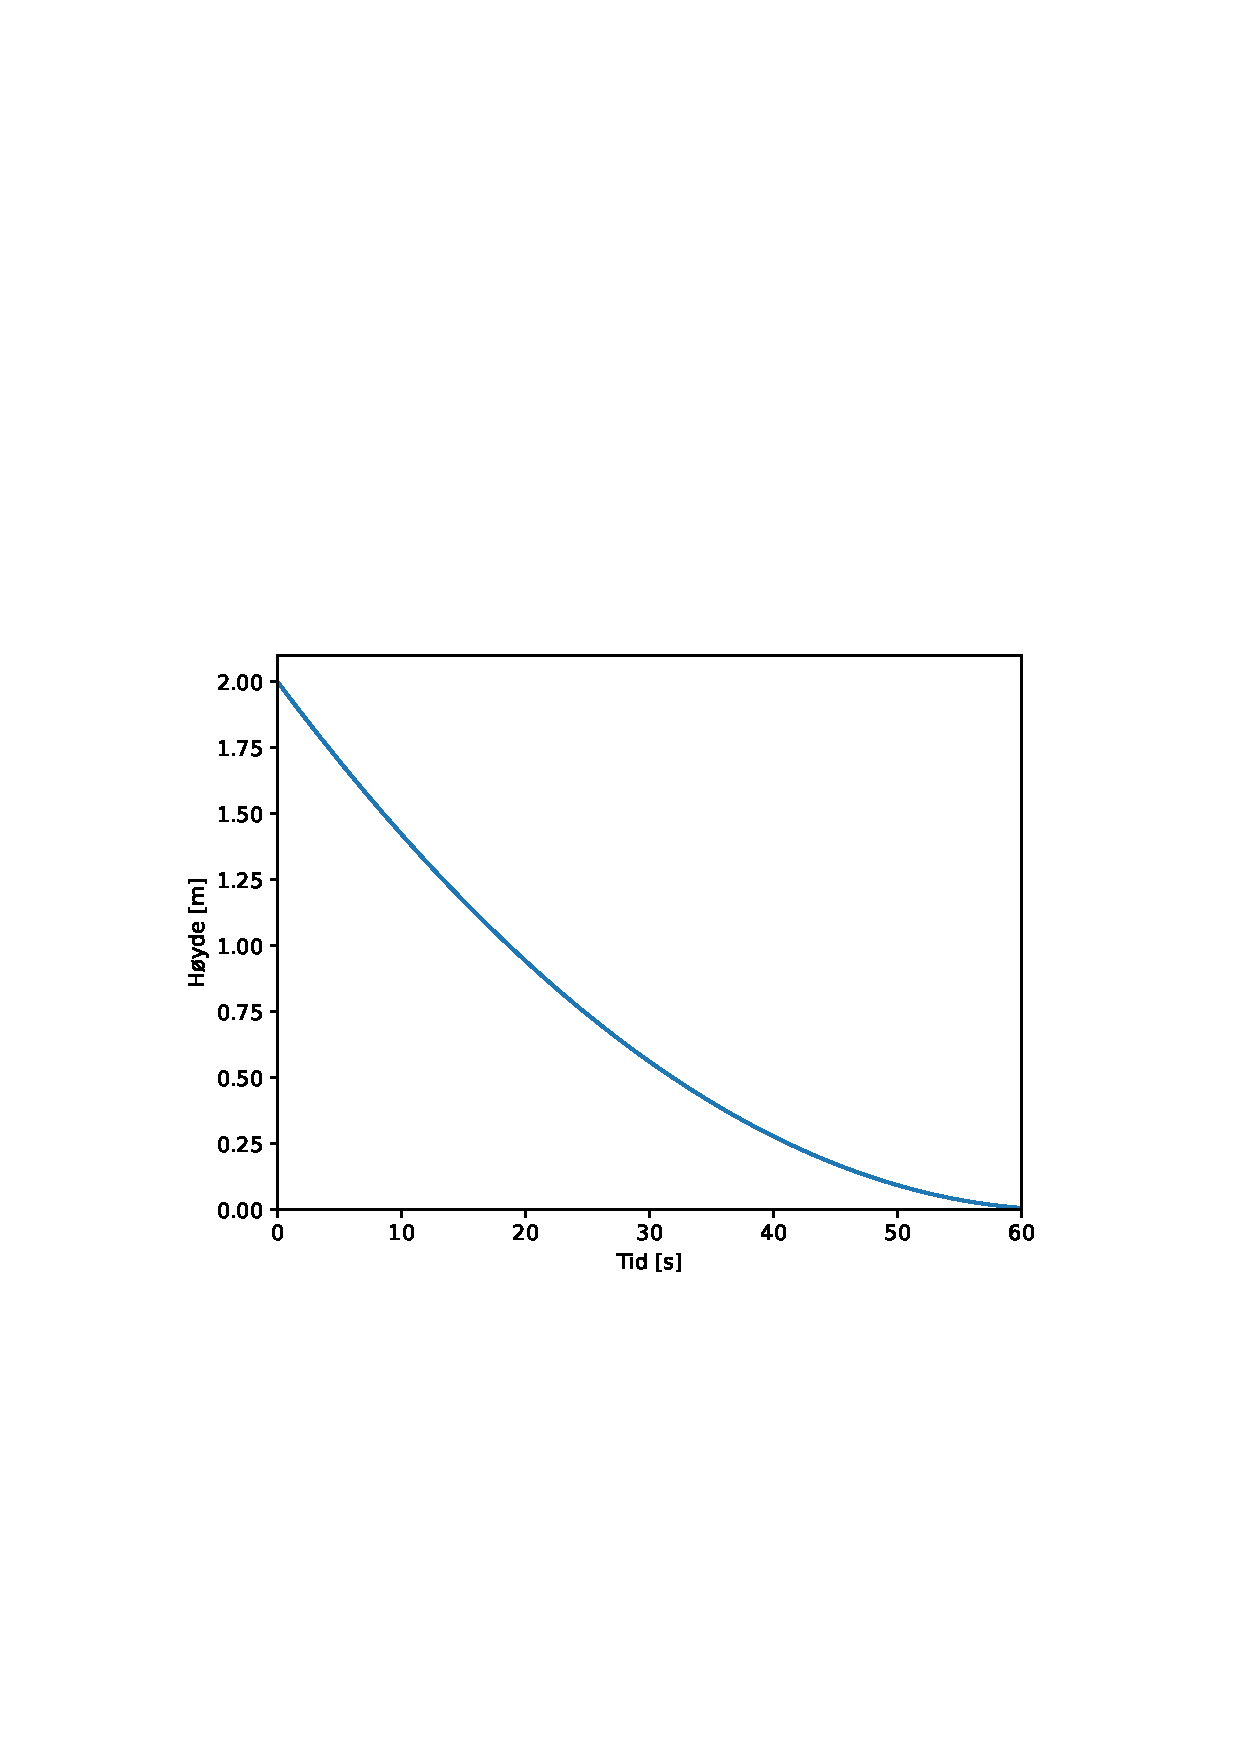
\includegraphics[scale=0.7]{Figures/tank.pdf}
    \caption{}
    \label{fig:tank}
\end{figure}

\begin{enumerate}
    \item Sett opp en ligning som viser høyden i tanken som funksjon av tid
    \item Bestem hastigheten for å sette ligningen på løsbar form
    \item Skriv et program som løser differensialligningen og plotter høyden som funksjon av tid
\end{enumerate}

\textbf{Løsningsforslag til punkt 1:} \\
Vi ønsker å finne ut hvor lang tid det tar å tømme den åpne tanken med vann. For å gjøre dette må vi først sette opp en enkel modell for systemet. Ved å bruke den generelle ligningen \cref{eq:akkumulering_generell} for massebevaring setter vi opp konserveringslikningene for masse som tidligere:
\begin{equation}
    \dot{m} = m_{inn} - m_{ut},
    \label{eq:mass_conservation}
\end{equation}
der $\dot{m}$ er hvordan massen i tanken endrer seg, mens $m_{inn}$ og $m_{ut}$ er henholdsvis massestrømmer inn og ut av tanken. Siden vi har interesse av å finne høyden til massen kan vi omformulere \eqref{eq:mass_conservation} i form av volum:
\begin{equation}
    \frac{d (\rho V)}{dt} = (\rho q)_{inn} - (\rho q)_{ut},
\end{equation}
der $\rho$ er massetettheten og $q$ er volumstrømmen. Siden massetettheten til vann er konstant, kan denne trekkes ut av den deriverte og strykes på begge sider:
\begin{equation}
    \frac{dV}{dt} = q_{inn} - q_{ut}
\end{equation}

Siden tanken vår kan beskrives som en sylinder kan vi sette inn volumet for en sylinder $V=\pi r^2h$. Når tanken tømmes vil væsken oppta et mindre volum av tanken, og det er høyden som endres etter hvert som tiden går. Det betyr at vi kan trekke $\pi r^2$ ut av den deriverte slik at
\begin{equation}
    \frac{dh}{dt} = \frac{1}{\pi r^2}(q_{inn} - q_{ut})
\end{equation}
Til slutt vil vi fjerne $q_{inn}$ siden det kun går masse ut av tanken, og det er da ingen volumstrøm inn. Merk at dette leddet kunne blitt fjernet tidligere i utledningen. Nå sitter vi igjen med en differensiallikning for endringen av høyden til tanken som funksjon av kun $t$ og $q_{ut}$. 
\begin{equation}
    \frac{dh}{dt} = -\frac{1}{\pi r^2} q_{ut}
    \label{eq:dh_dt_non_closed}
\end{equation}

\textbf{Løsningsforslag til punkt 2:} \\
Vi vet fortsatt ingen ting om $q_{ut}$, så vi kan enda ikke løse \eqref{eq:dh_dt_non_closed}. For enkelhetens skyld benytter vi oss av hastighetsuttrykket for rørstrømning
\begin{equation}
    q = vA,
    \label{eq:volume_from_velocity}
\end{equation}
der $v$ er hastigheten og $A$ er tverrsnittsarealet til røret. Deretter tar vi for oss Bernoulli som er kjent fra strømning fra våren i fjor
\begin{equation}
    \frac{1}{2}v_1^2 + gz_1 + \frac{p_1}{\rho} = \frac{1}{2}v_2^2 + gz_2 + \frac{p_2}{\rho}
\end{equation}
Vi velger å se på en strømlinje fra toppen av vannsøylen der hastigheten er 0 og trykker er $p_0=\SI{1}{\atm}\approx \SI{1}{\bar}$ I tillegg er trykket ved utløpet også $p_0\approx \SI{1}{\bar}$, siden vannet som kommer ut av utløpet også er i kontakt med lufta rundt. Ved å sette nullnivå ved utløpet og $z_1=h$ er utløpshastigheten dermed gitt av 
\begin{equation}
    v_2 = \sqrt{2gh}
    \label{eq:bernoulli_velocity}
\end{equation}
Ved å sette \eqref{eq:bernoulli_velocity} inn i \eqref{eq:volume_from_velocity}, og deretter sette resulatet inn i \eqref{eq:dh_dt_non_closed} får vi følgende uttrykk
\begin{equation}
    \frac{dh}{dt} = -\frac{1}{\pi r_{tank}^2} \sqrt{2gh}\frac{\pi}{4}d_{\text{rør}}^2
\end{equation}
Vi pynter litt på uttrykket og ender opp med den implementerbare likningen for tømmeprosessen
\begin{equation}
    \frac{dh}{dt} = -\left(\frac{d_\text{rør}}{d_{tank}}\right)^2 \sqrt{2gh}
    \label{eq:ODE_tank}
\end{equation}

\textbf{Løsningsforslag til punkt 3:} \\
For å løse differensiallikningen med programmering bruker vi parameterene gitt i tabell \ref{tab:tank_parameters}. \cref{eq:ODE_tank} kan beskrives som en første ordens differensiallikning og som vist i \cref{sec:numerisk_approksimasjon} kan vi approksimere en differensialligning ved bruk av Taylor rekker. 

\begin{lstlisting}[language=python]
#!/usr/bin/python
# -*- coding: utf-8 -*-

# =============== IMPORTS ============== #
import numpy as np
import matplotlib.pyplot as plt


# ============= PARAMETERS ============= #
d_pipe = 0.1            # Diameter for utløpsrør
d_tank = 1              # Diameter for tanken
g = 9.81                # Gravitasjonskonstant
h0 = 2                  # Starthøyde
dt = 0.1                # Steglengde
t0 = 0                  # Starttid
tN = 60                 # Sluttid
N = int((tN-t0)/dt + 1)  # Antall punkter


# ======== FUNCTION DEFINITIONS ======== #
def dhdt(h,t):
    # Høyresiden av likningen y' = f(h, t), med andre ord f(h, t)
    return -(d_pipe/d_tank)**2 * np.sqrt(2*g*h)

def euler(dt, h, t):
    # Numerisk finner neste y ved y_n+1 = y_n + h * f(h, t)
    return h + dt * dhdt(h, t)






def solve_ode():
    # Sett starttiden, det vil si initialtid
    t_current = t0
    
    # Lag vektorer som lagrer løsningen og tiden
    h = [h0]
    t = [t0]
    for _ in range(N):
        t_current += dt
        h_current = h[-1] # Hent siste element
        h_new = euler(dt, h_current, t) # Beregn neste høyde
        # Legg til tid og høyde i vektorer
        t.append(t_current)
        h.append(h_new)
    # Lag grafisk representasjon av høyden som funksjon av tid
    plt.plot(t, h)
    # Juster aksene
    plt.xlim(t0, tN)
    plt.ylim(0, 2.1)
    # Lag aksetitler
    plt.xlabel('Tid [s]')
    plt.ylabel('Høyde [m]')
    # Lagre bildet i høy kvalitet
    plt.savefig('tank.eps', format='eps', dpi=400)
    # Vis plottet :)
    plt.show()
    plt.close()


# ========= PROGRAM EXECUTION ========== #
if __name__ == '__main__':
    solve_ode()

\end{lstlisting}

Når vi kjører koden så får vi ut plottet i \cref{fig:ODE_tank_plot}.

\begin{figure}[h!]
    \centering
    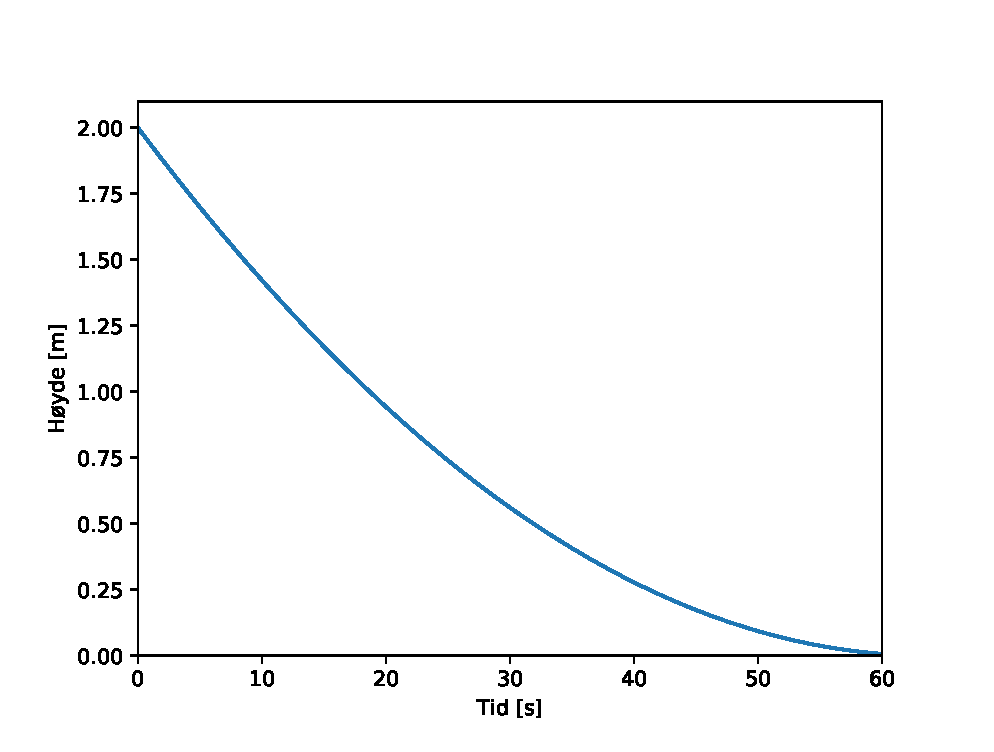
\includegraphics[scale=0.8]{Text/tank.eps}
    \caption{}
    \label{fig:ODE_tank_plot}
\end{figure}

\newpage
\subsection{Klasser og objekter}
Til nå har dere ofte programmert i en fil med definering av variabler øverst i filen og så skrevet viktige funksjonener under. I IT-verdenen er dette kronglete siden et program kan trenge flere titusen linjer med koder så vi må ha et system for å sortere koden. Samtidig vil operasjoner i programmet gjenta seg og vi ønsker ikke å skrive en kode flere ganger. Av den grunn er objektorientert programmering fantastisk siden vi kan generalisere hvordan en del av koden skal oppføre seg i forhold til en annen del. Formelt sett er klasser et overordnet rammesystem for hvordan objekter kommuniserer sammen. Det kan være alt fra hvordan en bil ser ut til hvordan et matematisk system fungerer. Før dere blir mer forvirret trekker vi fram et eksempel på klasser og objekter.

\subsubsection{Eksempel: Katter og hunder}
Tenk deg at du har lager et dataspill med en åpen verden og sjefen din ber deg om å fylle verdenen med katter. Du tenker deg om og kommer fram til følgende konklusjon: Alle kattene i denne verdenen har et navn og har fire bein. Istedet for å programmere dette for hver eneste katt lager vi et generelt rammeverk som gjelder alle katter.

\begin{figure}[H]
    \centering
    \includegraphics[scale=0.5]{Figures/Klasser_katt.png}
    \caption{En visualisering av klassen $"$Katt$"$.}
    \label{fig:Katte_boks}
\end{figure}

Når vi lager et rammeverk for alle kattene kan vi fylle verdenen vår med mange katteobjekter. Det vil si at i verdenen vår har vi mange forskjellige katte-objekter, men alle katte-objektene tilhører klassen ``Katt'' og hvert katte-objekt vil ha et navn og fire bein. Ved bruk av python som programmeringspråk skriver vi klassen for katt.\\[0.5cm]
\textbf{Del 1 (Kode):}
\begin{lstlisting}[language=python]
class Katt: #Klassen katt
    #Medlemsvariabler
    antall_ben = 4 
    navn ="" #Default navn
    
    #Constructor
    def __init__(self, navn): #Lager Katte-objektet med spesifisert navn
        self.navn = navn #Endrer navnet til katten fra "" til det vi spesifiserte

\end{lstlisting}
\textbf{Del 2 (Konsoll):}
\begin{lstlisting}[language=python]
>>> katten_butte = Katt("Butte") #Lager et katteobjekt med variabelnavn "katten_butte"
>>> print(katten_butte.navn) 
Butte
>>> print(katten_butte.antall_ben) 
4
\end{lstlisting}

En liten forklaring på hva som skjer.

``\twound{init}\twound{\text{ }}(self,navn)'' er en konstruktør for et katte-objekt. init kommer fra det engelske ordet ``initial''. Når vi skal lage et et katteobjekt må vi kalle på konstruktøren vår. Ved å kalle på kontruktøren lager python et tomt objekt og sender det til oss i form av ``self''. Self er på mange måter ``Seg selv'' så når vi bruker self snakker vi om det spesifikke katte-objektet. Konstruktøren tar også inn et navn som vi må spesifisere. Vi kunne ha programmert konstruktøren til å ta inn antall bein også, men siden en katt alltid har 4 bein så gir det ingen mening å la brukeres bestemme hvor mange bein et katte-objekt skal ha. På linje 1 i Del 2 lager vi et objekt som vi kaller ``katten\_butte'' som vi spesifiserer skal ha navnet ``Butte''. Navn og antall bein til katten er en instans av klassen vår. Det vil si ``Egenskaper'' til katte-objektet. Her er det viktig å skille mellom variabelnavnet på objektet og instansen til objektet som er vi har valgt å kalle ``navn''.

Sjefen vår er ikke helt fornøyd med at spillverdenen bare består av katter. Han ber oss om å legge til hunder i tillegg til kattene og hundene skal kunne bjeffe.

\begin{figure}[H]
    \centering
    \includegraphics[scale=0.5]{Figures/Klasser_hund.png}
    \caption{En visualisering av klassen ``Hund''.}
    \label{fig:klasse_hund}
\end{figure}

Hunden har de samme medlemsvariablene som en katt, men skal i tillegg ha medlemsfunksjonen å bjeffe. Dette gjør vi ved å lage det som kalles en medlemsfunksjon til klassen. En funksjon som bare klassen $"$Hund$"$ kan benytte seg av.\\[0.5cm]
\textbf{Del 1 (Kode):}
\begin{lstlisting}[language=python]
class Hund: #Klassen Hund
    #Medlemsvariabler
    antall_ben = 4 
    navn ="" #Default navn
    
    #Constructor
    def __init__(self, navn): #Lager hunde-objektet med spesifisert navn
        self.navn = navn #Endrer navnet til hunden fra "" til det vi spesifiserte
    #Medlemsfunksjon
    def bjeffe(self): 
        print("BARK BARK")
\end{lstlisting}
\textbf{Del 2 (Konsoll):}
\begin{lstlisting}[language=python]
>>> Hunden_tara = Hund("Tara") #Lager et Hundeobjekt med variabelnavn "Hunden_tara"
>>> print(Hunden_tara.navn) 
Tara
>>> Hunden_tara.bjeffe() #Kaller bjeffefunksjonen
BARK BARK
\end{lstlisting}

Nå har vi en klasse for Hund og for Katt som alle objekter i spillverdenen vår må følge. En klasse er et strengt rammeverk i form av at et objekt ikke kan gjøre annet enn det klassen tillater. Det vil si at hvis vi prøver å skrive katten\_butte.bjeffe() så får vi feilmelding siden klassen Katt, som katten\_butte er et objekt av, ikke har en funksjon som heter bjeffe(). 

\clearpage
\subsection{Superklasser, subklasser og arv}
I mange tilfeller vil man ha klasser som har de samme medlemsvariablene og samme medlemsfunksjonene. Istedet for å definere de samme funksjonene til hver klasse er det smartere å la en klasse arve medlemsfunksjoner og medlemsvariabler fra det vi kaller en superklasse. 

\subsubsection{Eksempel: Mange forskjellige dyr}
Sjefen vår kommer inn og sier at vi også skal ha kuer, griser, hester og mange andre forskjellige dyr i spillverdenen vår. Vi oppdager at dette blir mye repetisjon av kode som vi må spesifisere for hver klasse. Hund og katt hadde begge 4 ben og et navn. Her kan vi koble disse to klassene til en superklasse som vi kaller Dyr. Hund og Katt blir da subklasser av superklassen Dyr.\\[2cm]

\begin{figure}[H]
    \centering
    \includegraphics[scale=0.5]{Figures/Klasser_Dyr.png}
    \caption{En visualisering av superklassen Dyr med Katt og Hund som subklasser.}
    \label{fig:uperklasse}
\end{figure}
\clearpage
\begin{lstlisting}[language=python]
class Dyr(): # Klassen Dyr
    #Medlemsvariabler for alle dyre-objekter
    antall_ben = 4
    navn = ""
    #Contructor for dyre-objekter
    def __init__(self, navn):
        self.navn = navn

class Katt(Dyr): # Klassen Katt, arver fra klassen Dyr
    #Medlemsfunksjoner
    def mjaue(self):
        print("MJAAAAU")
        
    def __init__(self,navn): #Spesifiserer construktor for Katte-klassen
        super().__init__(self,navn) #Kaller superklassen sin constructor


class Hund(Dyr):  # Klassen Hund, arver fra klssen Dyr
    #Medlemsfunksjon
    def bjeffe(self):
        print("Walla bruh, bjeff litt for meg da")
\end{lstlisting}

Som du ser i koden over så har klassen Katt en spesifisert konstruktør mens Hund har ingen. I realiteten er det ingen forskjell mellom klassene siden linje 15 kaller på konstruktøren til Dyr hvorav Katt vil automatisk kalle på konstruktøren. Denne kalles automatisk siden Katt arver konstruktøren til klassen Dyr. Vi valgte å ta med linje 14 og 15 for å vise deg hvordan du kan definere din egen konstruktører for subklasser. Dette er nyttig å kunne når subklasser skiller seg fra superklasser.

\textbf{Ekstra}: \\
Under er koden for filen $"$Min\_python\_fil.py$"$
\begin{lstlisting}[language=python]
if __name__ == "__main__":
    print("Dette er hovedskriptet")
\end{lstlisting}

Linje 1 i koden over er litt merkelig å forstå, men tanken er at hvis du kaller på den spesifikke filen  $"$Min\_python\_fil.py$"$ så vil betingelsen til if-setningen gi ut True som gjør at linje 2 vil kjøre.

\begin{lstlisting}
>>> python Min_python_fil.py
Dette er hovedskriptet
\end{lstlisting}
 Vi ønsker å gjøre dette er fordi filen kan importeres fra andre filer. Hvis vi kjører en annen fil som importerer  $"$Min\_python\_fil.py$"$, så vil ikke if-betingelsen godkjennes.  

